\documentclass[conference,compsoc]{IEEEtran}
\usepackage{./macros}

\begin{document}
\vspace{3cm}
\title{CS5300 Assignment 2}
\author{Gautam Singh\\CS21BTECH11018}
\maketitle
\tableofcontents

\bigskip

\begin{abstract}
    This report analyzes various techniques implemented for a multithreaded
    solution to computing the sparsity of a square matrix using various
    multithreading libraries, namely pthreads (POSIX Threads) and OpenMP (Open
    Multi-Processing). The sparsity of a matrix is defined as the number of zero
    entries in the matrix. The report is organized as follows. In
    \autoref{sec:prog-design}, we describe the low-level program design on which
    our experiments are run. In \autoref{sec:results-and-analysis}, we present
    the results of various experiments and analyze them. Finally, we conclude
    the report in \autoref{sec:conclusion}.  
\end{abstract}

\section{Program Design}
\label{sec:prog-design}

We describe the low-level program design of our C++ implementation used to
compute the sparsity of the input matrix.

\subsection{Command Line Options}
\label{subsec:cmd-line-options}

The program takes various arguments that can be found in the \texttt{help}
function of the code. In particular, the technique and library to be used is
specified using the command line and parsed during execution. Runner functions
for each technique have been implemented. Based on the chosen technique, all
threads run one of the implemented functions to compute the sparsity of the
matrix.

\subsection{Thread Information}
\label{subsec:thread-infos}

Each thread has its own \texttt{ThreadInfo} struct which is defined in
\autoref{code:ThreadInfo}.

\begin{listing}[!ht]
\inputminted{cpp}{codes/ThreadInfo.cpp}
\caption{The ThreadInfo struct.}
\label{code:ThreadInfo}
\end{listing}

On executing the runner function, the sparsity computed by this thread is stored
in the field \texttt{res}. For static methods, the \texttt{id} field can be used
to compute the allocation of rows to this thread. These structs are stored in a
global array accessible to any runner function.

\subsection{Runner Functions}
\label{subsec:runners}

Runner functions are created for each combination of method (chunk, mixed and
dynamic) and library (pthreads and OpenMP). The naming convention followed for
these functions is \texttt{<LIB>\_<TECH>Runner}, where \texttt{LIB} is the
library to be used and \texttt{TECH} is the technique to be used.

Runner functions have the signature \texttt{void *()(void *)}. That is, runners
receive a generic pointer and return a generic pointer. We create a hash table
(using the C++ \texttt{unordered\_map} container) mapping the string
\texttt{<LIB>\_<TECH>} obtained from the command line arguments to its
corresponding runner function pointer to be used, or to output an error message
in case of invalid input.

\subsection{Pthreads Runners}
\label{subsec:pthreads}

For runner functions implemented using the pthreads API, threads are created and
joined in the main function using \texttt{pthread\_create} and
\texttt{pthread\_join}. For compatability with the API, runner functions have
the signature described in \autoref{subsec:runners}. Threads are passed a
generic pointer to the respective \texttt{ThreadInfo} struct, since thread IDs
can be arbitrary. To implement the dynamic methods, the dynamic technique runner
makes use of the atomic shared counter described in \autoref{subsec:counter}.

\subsection{OpenMP Runners}
\label{subsec:openmp}

In contrast to the runner functions implemented for pthreads, runner functions
implemented using OpenMP are much smaller in code size, due to the following
reasons.

\begin{enumerate}
    \item Thread IDs alloted to OpenMP threads are 0-indexed, thus we can use
    them directly as an index to the global \texttt{ThreadInfo} array. It is for
    this reason that we pass a null pointer to the OpenMP runners. 
    \item Various OpenMP \texttt{pragma} directives can be used to implement the
    required computation technique. In particular, the \texttt{schedule}
    directive determines the method in which work should be allocated to
    threads. Among many other schedules, we use either \texttt{static} or
    \texttt{dynamic} scheduling, with chunk size being specified where needed.
    By default, \texttt{static} scheduling allocates roughly equal work to all
    threads.
    
    Since these directives take care of work allocation, we do not need to use
    any shared counters or thread IDs to determine the work of each thread. 
\end{enumerate}

\subsection{Atomic Shared Counters}
\label{subsec:counter}

For the dynamic row allocation technique in pthreads, we create a
\texttt{Counter} class, whose memebers and methods are defined in
\autoref{code:Counter}. Full implementation details can be found in the source
code, and are omitted for brevity.

\begin{listing}[!ht]
\inputminted{cpp}{codes/Counter.cpp}
\caption{The \texttt{Counter} class.}
\label{code:Counter}
\end{listing}

The \texttt{Counter} class is a template class, meaning one can instantiate a
counter using integral data-types of various sizes and signedness. For our
purposes, we use a 64-bit unsigned integer as the integral data type. The atomic
operations are provided by the \texttt{atomic} class in the C++ standard
library. The following methods are implemented:

\begin{enumerate}
    \item \texttt{T get()}: Read the current value stored in the counter
    atomically. Threads use this to check how many rows or blocks have their
    sparsity computed.
    \item \texttt{T getAndIncrement(T inc)}: Read the current value and then
    increment the counter by \texttt{inc}. Threads use this to get the id of the
    row or block on which sparsity is to be computed. 
\end{enumerate}

\subsection{Timing}
\label{sec:timing}

The \texttt{chrono} class provided by the C++ library was used to measure
execution time. Specifically, the time taken from creation of threads to their
joining was measured in milliseconds. 

\section{Results and Analysis}
\label{sec:results-and-analysis}

The following experiments have been performed on an Intel i9-11900H 8-core
16-thread CPU. We analyze the variation of execution time on varying different
parameters one-by-one.

\subsection{Time vs. Size}
\label{subsec:time-vs-size}

\begin{figure}[!ht]
    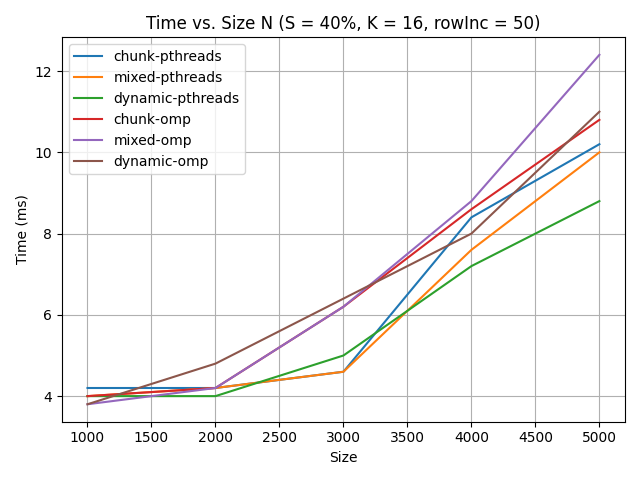
\includegraphics[width=\columnwidth]{images/exp1.png}
    \caption{Execution time vs. matrix size for various techniques.}
    \label{fig:exp-1}
\end{figure}

\autoref{fig:exp-1} shows the execution time for various methods as matrix size
\(N\) changes. We set the number of threads \(K = 16\), row increment \(rowInc =
50\) and sparsity \(S = 40\%\). The total number of zero elements is shown in
\autoref{tab:exp1-table}. We observe the following.

\begin{table}[!ht]
    \begin{tabularx}{\columnwidth}{|Y|Y|Y|Y|Y|Y|}
        \hline
        \textbf{Size \(N\)} & 1000 & 2000 & 3000 & 4000 & 5000 \\
        \hline
        \textbf{No. of Zeros (\(\times 10^6\))} & 0.4 & 1.6 & 3.6 & 6.4 & 10 \\
        \hline
    \end{tabularx}
    \caption{Number of zeros for 40\% sparsity as a function of matrix size.}
    \label{tab:exp1-table}
\end{table}

\begin{enumerate}
    \item Execution time for all methods increases with size roughly
    quadratically.
    \item Within a library, dynamic methods perform better than static methods
    on average. This is because the zero entries in the matrix are randomly
    dispersed, so a dynamic method ensures a fairer work division among the
    threads.
    \item Pthreads outperforms OpenMP on all techniques.
\end{enumerate}

\subsection{Time vs. Number of Threads}
\label{subsec:exp2}

\begin{figure}[!ht]
    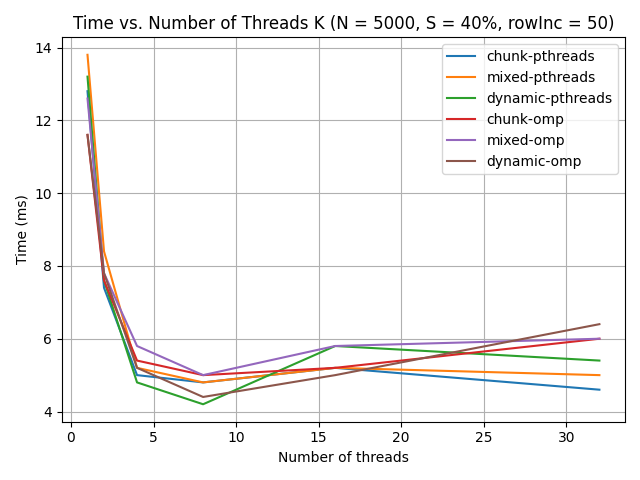
\includegraphics[width=\columnwidth]{images/exp2.png}
    \caption{Execution time vs. number of threads for various techniques.}
    \label{fig:exp-2}
\end{figure}

\autoref{fig:exp-2} shows the execution time for various methods as the number
of threads increases. We set \(N = 5000\), \(S = 40\%\) and \(rowInc = 50\). The
following observations can be made.

\begin{enumerate}
    \item The best performance occurs when using 8 threads. As the number of
    threads increases, initially the execution time reduces drastically.
    However, on still increasing the number of threads, the delay during context
    switches dominates, thus the total execution time increases.
    \item For larger number of threads, static methods dominate on pthreads,
    since there may be more competition among threads in incrementing the atomic
    shared counter. However, for OpenMP, the dynamic method is faster even for a
    larger number of threads, suggesting a different method of dynamic row
    allocation.
    \item The optimal runtimes for dynamic methods are the best (at 8 threads).
    \item Pthreads outperforms OpenMP in this setting as well.
\end{enumerate}

\subsection{Time vs. Sparsity}
\label{subsec:exp3}

\begin{figure}[!ht]
    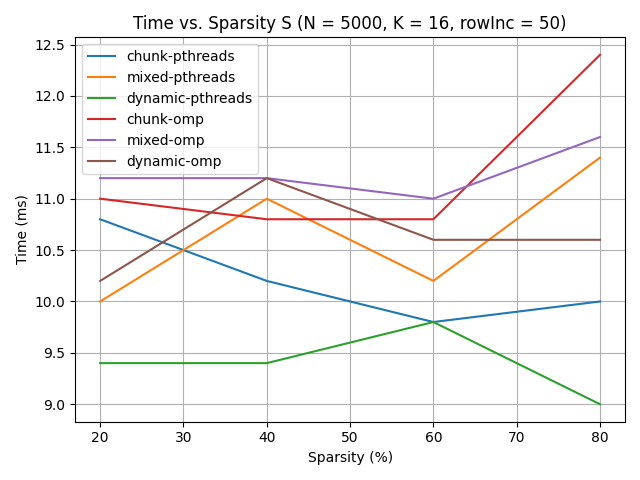
\includegraphics[width=\columnwidth]{images/exp3.png}
    \caption{Execution time vs. sparsity for various techniques.}
    \label{fig:exp-3}
\end{figure}

\autoref{fig:exp-3} shows the execution time for various methods as the sparsity
of the matrix increases. We set \(N = 5000\), \(K = 16\) and \(rowInc = 50\).
The number of zeros computed in each case are depicted in
\autoref{tab:exp3-table}. The following observations can be made.

\begin{table}[!ht]
    \begin{tabularx}{\columnwidth}{|Y|Y|Y|Y|Y|}
        \hline
        \textbf{Sparsity} & 20\% & 40\% & 60\% & 80\% \\
        \hline
        \textbf{No. of Zeros (\(\times 10^6\))} & 5 & 10 & 15 & 20 \\
        \hline
    \end{tabularx}
    \caption{Number of zeros for various sparsity levels where \(N = 5000\).}
    \label{tab:exp3-table}
\end{table}

\begin{enumerate}
    \item Static methods perform comparatively more poor when the sparsity
    increases. This is because the sparsity is distributed at random, resulting
    in improper load balancing on using static methods. In such cases, dynamic
    methods perform better and should be preferred. Thus, for both libraries,
    dynamic methods perform the best.
    \item Pthreads outperforms OpenMP on all methods here. In particular,
    pthreads outperforms OpenMP by about 1.5 milliseconds at 80\% sparsity on
    dynamic allocation.
\end{enumerate}

\subsection{Time vs. Row Increment}
\label{subsec:exp4}

\begin{figure}[!ht]
    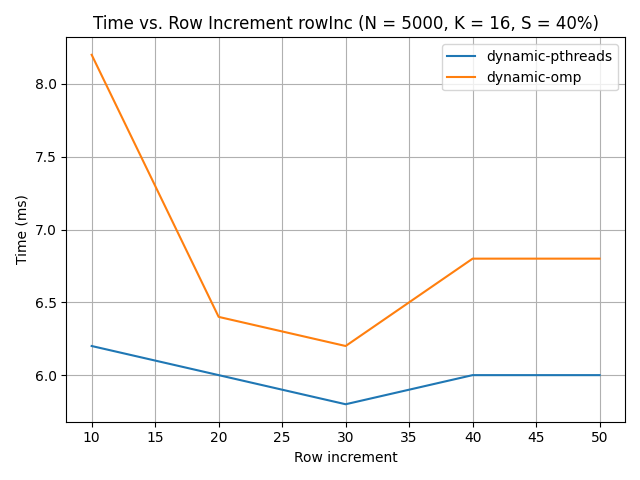
\includegraphics[width=\columnwidth]{images/exp4.png}
    \caption{Execution time vs. Row increments for dynamic allocation methods.}
    \label{fig:exp-4}
\end{figure}

\autoref{fig:exp-4} shows the execution time for various dynamic methods as the
row increments change. We set \(N = 5000\), \(S = 40\%\) and \(K = 16\). The
following observations can be made.

\begin{enumerate}
    \item The optimal row increment for this setting turns out to be \(rowInc =
    30\) for both libraries.
    \item The initial decrease in runtime as row increment increases is more
    drastic in OpenMP than in pthreads. In both cases, it is due to cache
    locality being exploited.
    \item However, runtime then increases with increasing row increment because
    it is too large, leading to possibly improper load balancing as the chunks
    are too large.
    \item Pthreads again outperforms OpenMP over all row increments.
\end{enumerate}

\section{Conclusion}
\label{sec:conclusion}

We conclude that for many cases, dynamic methods of work allocation to threads
is better, especially since the sparsity of the matrix is randomly distributed.
Further, Pthread performed better than OpenMP on all experiments, even with
using our constructs such as the atomic shared counter. This might be because
the Pthreads API is lower level than OpenMP, and thus more performant for this
task. OpenMP, on the other hand, is suited for portable code and faster
development.

\end{document}